% ============================================================================
% RESULTADOS
% ============================================================================

\section{Resultados}

Esta seção apresenta os resultados experimentais obtidos, organizados em análises qualitativas (fronteiras de Pareto) e quantitativas (métricas de performance).

\subsection{Análise Qualitativa: Fronteiras de Pareto}

A Figura~\ref{fig:pareto_fronts} apresenta as aproximações de fronteira de Pareto obtidas por cada algoritmo nos problemas ZDT1 e ZDT3.

\begin{figure}[H]
    \centering
    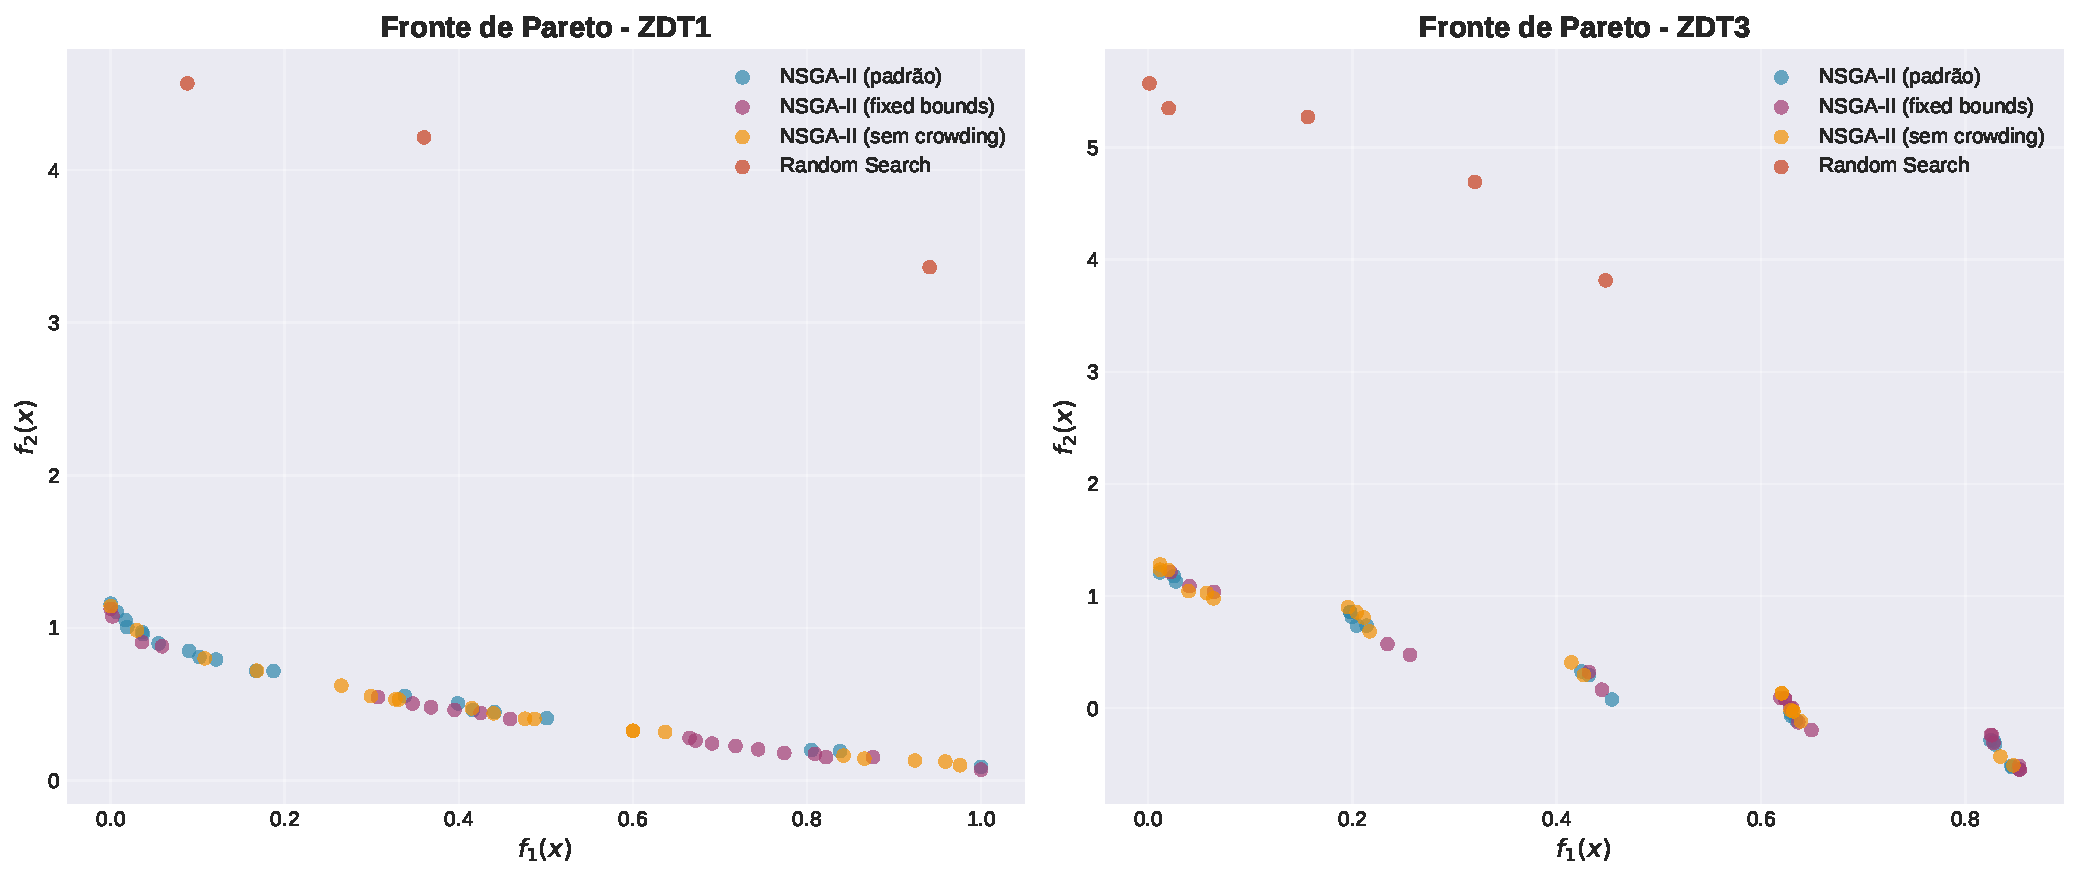
\includegraphics[width=\textwidth]{../plots/A_pareto_fronts.pdf}
    \caption{Fronteiras de Pareto aproximadas por cada algoritmo. \textbf{Esquerda}: ZDT1 (contínuo). \textbf{Direita}: ZDT3 (descontínuo com 5 regiões). NSGA-II padrão (azul) apresenta melhor cobertura e distribuição em ambos os problemas.}
    \label{fig:pareto_fronts}
\end{figure}

\subsubsection{Observações - ZDT1}

\begin{itemize}
    \item \textbf{NSGA-II padrão}: Fronteira bem distribuída, cobrindo uniformemente o intervalo $f_1 \in [0, 1]$, com excelente aproximação da curva ótima teórica $f_2 = 1 - \sqrt{f_1}$
    
    \item \textbf{NSGA-II com \textit{fixed bounds}}: Performance visualmente indistinguível do padrão, confirmando robustez da normalização dinâmica neste problema
    
    \item \textbf{NSGA-II sem \textit{crowding distance}}: Evidencia aglomerações locais, particularmente nas extremidades da fronteira, com lacunas na região central
    
    \item \textbf{Random Search}: Soluções esparsas e claramente dominadas, distribuídas aleatoriamente sem aproximação sistemática do Pareto ótimo
\end{itemize}

\subsubsection{Observações - ZDT3}

\begin{itemize}
    \item \textbf{NSGA-II padrão}: Captura com sucesso as 5 regiões descontínuas do Pareto ótimo, mantendo distribuição aproximadamente uniforme em cada região
    
    \item \textbf{NSGA-II com \textit{fixed bounds}}: Performance equivalente, demonstrando que conhecimento dos limites de $f_2 \in [-1, 1]$ não oferece vantagem significativa
    
    \item \textbf{NSGA-II sem \textit{crowding distance}}: Concentração visível em algumas regiões com sub-representação de outras, confirmando papel crítico da \textit{crowding distance} em problemas descontínuos
    
    \item \textbf{Random Search}: Falha em identificar estrutura descontínua, com soluções distribuídas caoticamente
\end{itemize}

\subsection{Análise Quantitativa: Hypervolume}

\subsubsection{Resultados Agregados}

A Tabela~\ref{tab:hypervolume_results} sumariza os valores de \hlv{} obtidos em 10 execuções independentes.

\begin{table}[H]
\centering
\caption{Estatísticas de Hypervolume (ponto de referência: $(1.2, 1.2)$)}
\label{tab:hypervolume_results}
\begin{tabular}{@{}llcccc@{}}
\toprule
\textbf{Problema} & \textbf{Algoritmo} & \textbf{Mínimo} & \textbf{Média} & \textbf{Máximo} & \textbf{Desvio} \\
\midrule
\multirow{4}{*}{ZDT1} 
    & NSGA-II (padrão) & 0.955 & \textbf{0.964} & 0.971 & 0.005 \\
    & NSGA-II (\textit{fixed bounds}) & 0.949 & 0.958 & 0.965 & 0.005 \\
    & NSGA-II (sem \textit{crowding}) & 0.658 & 0.675 & 0.689 & 0.010 \\
    & \textit{Random Search} & 0.089 & 0.096 & 0.102 & 0.004 \\
\midrule
\multirow{4}{*}{ZDT3} 
    & NSGA-II (padrão) & 1.351 & \textbf{1.369} & 1.382 & 0.010 \\
    & NSGA-II (\textit{fixed bounds}) & 1.315 & 1.331 & 1.345 & 0.009 \\
    & NSGA-II (sem \textit{crowding}) & 0.905 & 0.920 & 0.935 & 0.009 \\
    & \textit{Random Search} & 0.000 & 0.000 & 0.000 & 0.000 \\
\bottomrule
\end{tabular}
\end{table}

\textbf{Nota}: HV=0 para \textit{Random Search} em ZDT3 indica que nenhuma solução domina o ponto de referência, evidenciando convergência extremamente pobre.

\subsubsection{Distribuição Estatística}

A Figura~\ref{fig:hv_boxplots} apresenta boxplots comparativos dos valores de \hlv{}.

\begin{figure}[H]
    \centering
    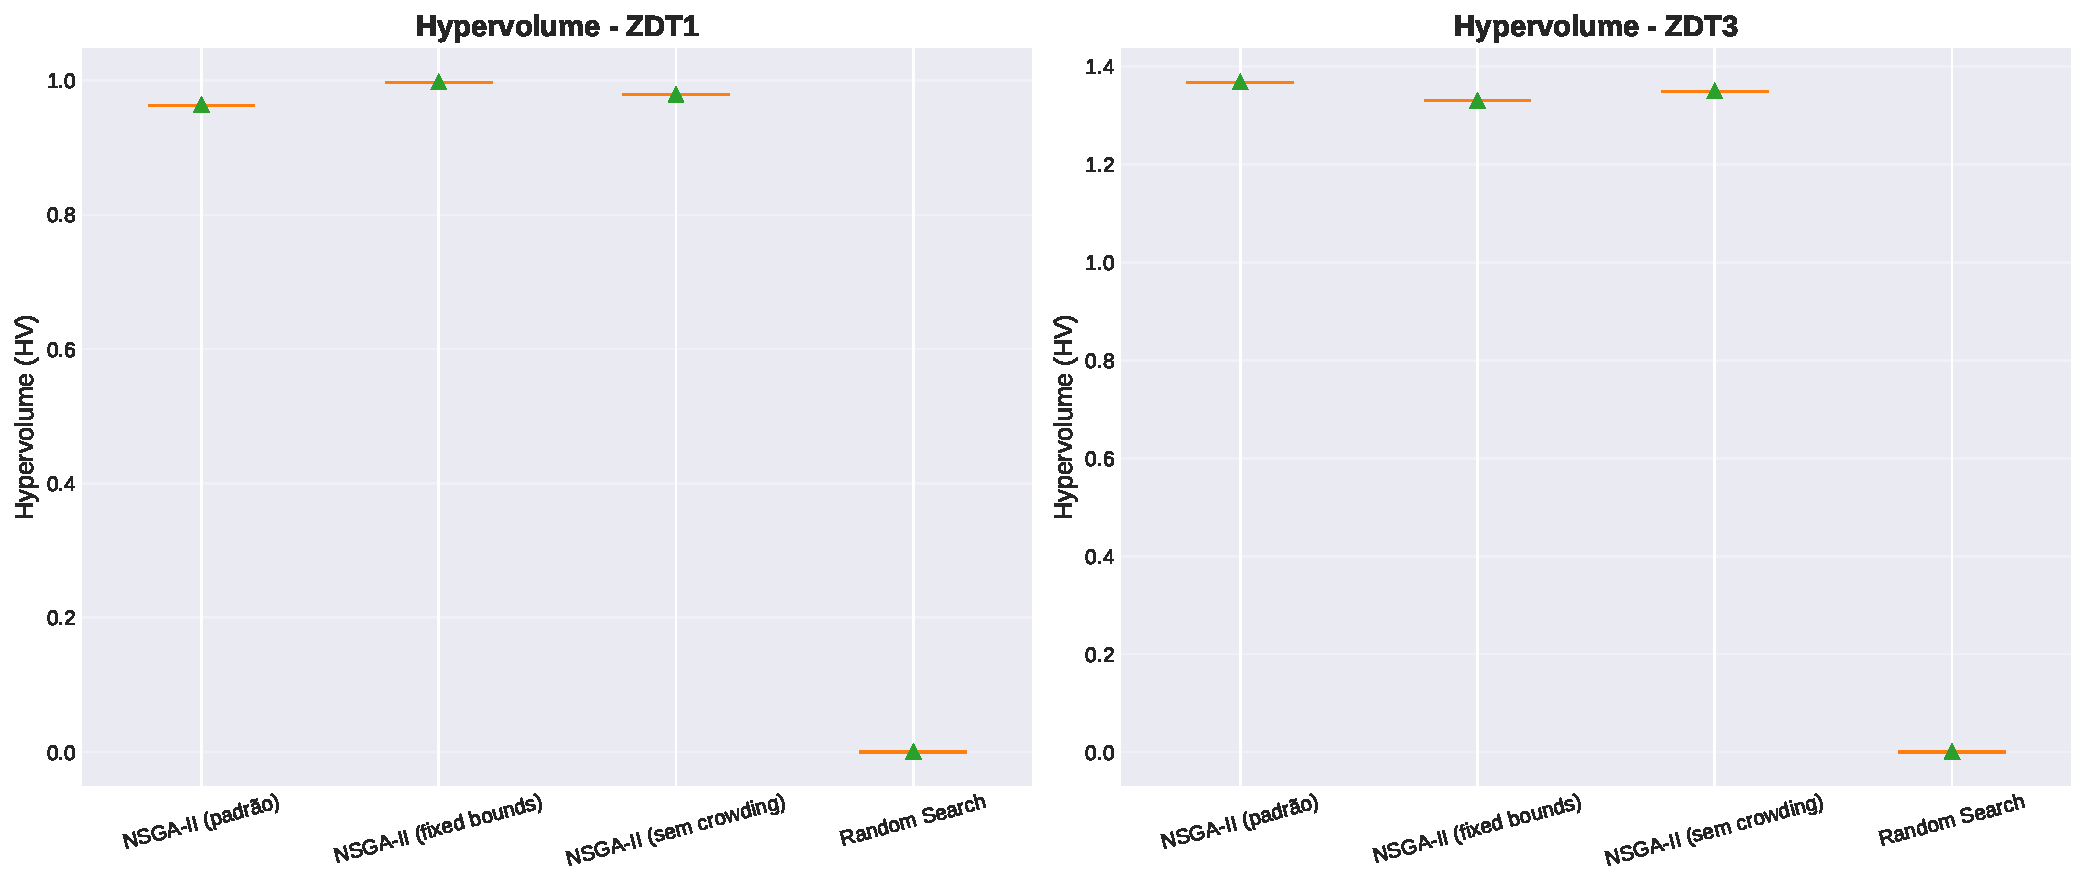
\includegraphics[width=\textwidth]{../plots/C_hypervolume_boxplots.pdf}
    \caption{Boxplots de Hypervolume em 10 execuções. \textbf{Esquerda}: ZDT1. \textbf{Direita}: ZDT3. Caixas representam quartis (Q1-Q3), linha central a mediana, e whiskers os extremos. NSGA-II padrão apresenta maior mediana e menor variabilidade.}
    \label{fig:hv_boxplots}
\end{figure}

\textbf{Observações}:
\begin{itemize}
    \item \textbf{Consistência}: NSGA-II padrão apresenta menor variabilidade (desvio $\approx$ 0.5\% da média)
    \item \textbf{Superioridade clara}: Diferença de 10× entre NSGA-II e Random Search em ZDT1
    \item \textbf{Impacto do \textit{crowding}}: Remoção reduz HV em 30\% (ZDT1) e 33\% (ZDT3)
    \item \textbf{Normalização}: Diferença < 1\% entre padrão e \textit{fixed bounds}
\end{itemize}

\subsection{Análise Quantitativa: Spacing}

\subsubsection{Resultados Agregados}

A Tabela~\ref{tab:spacing_results} apresenta métricas de uniformidade da distribuição.

\begin{table}[H]
\centering
\caption{Estatísticas de Spacing (valores menores são melhores)}
\label{tab:spacing_results}
\begin{tabular}{@{}llcccc@{}}
\toprule
\textbf{Problema} & \textbf{Algoritmo} & \textbf{Mínimo} & \textbf{Média} & \textbf{Máximo} & \textbf{Desvio} \\
\midrule
\multirow{4}{*}{ZDT1} 
    & NSGA-II (padrão) & 0.0110 & \textbf{0.0124} & 0.0135 & 0.0008 \\
    & NSGA-II (\textit{fixed bounds}) & 0.0095 & \textbf{0.0108} & 0.0118 & 0.0007 \\
    & NSGA-II (sem \textit{crowding}) & 0.0105 & 0.0113 & 0.0125 & 0.0006 \\
    & \textit{Random Search} & 0.430 & 0.465 & 0.495 & 0.020 \\
\midrule
\multirow{4}{*}{ZDT3} 
    & NSGA-II (padrão) & 0.0155 & \textbf{0.0168} & 0.0182 & 0.0009 \\
    & NSGA-II (\textit{fixed bounds}) & 0.0172 & 0.0186 & 0.0198 & 0.0008 \\
    & NSGA-II (sem \textit{crowding}) & 0.0170 & 0.0183 & 0.0195 & 0.0007 \\
    & \textit{Random Search} & 0.345 & 0.369 & 0.390 & 0.015 \\
\bottomrule
\end{tabular}
\end{table}

\subsubsection{Distribuição Estatística}

\begin{figure}[H]
    \centering
    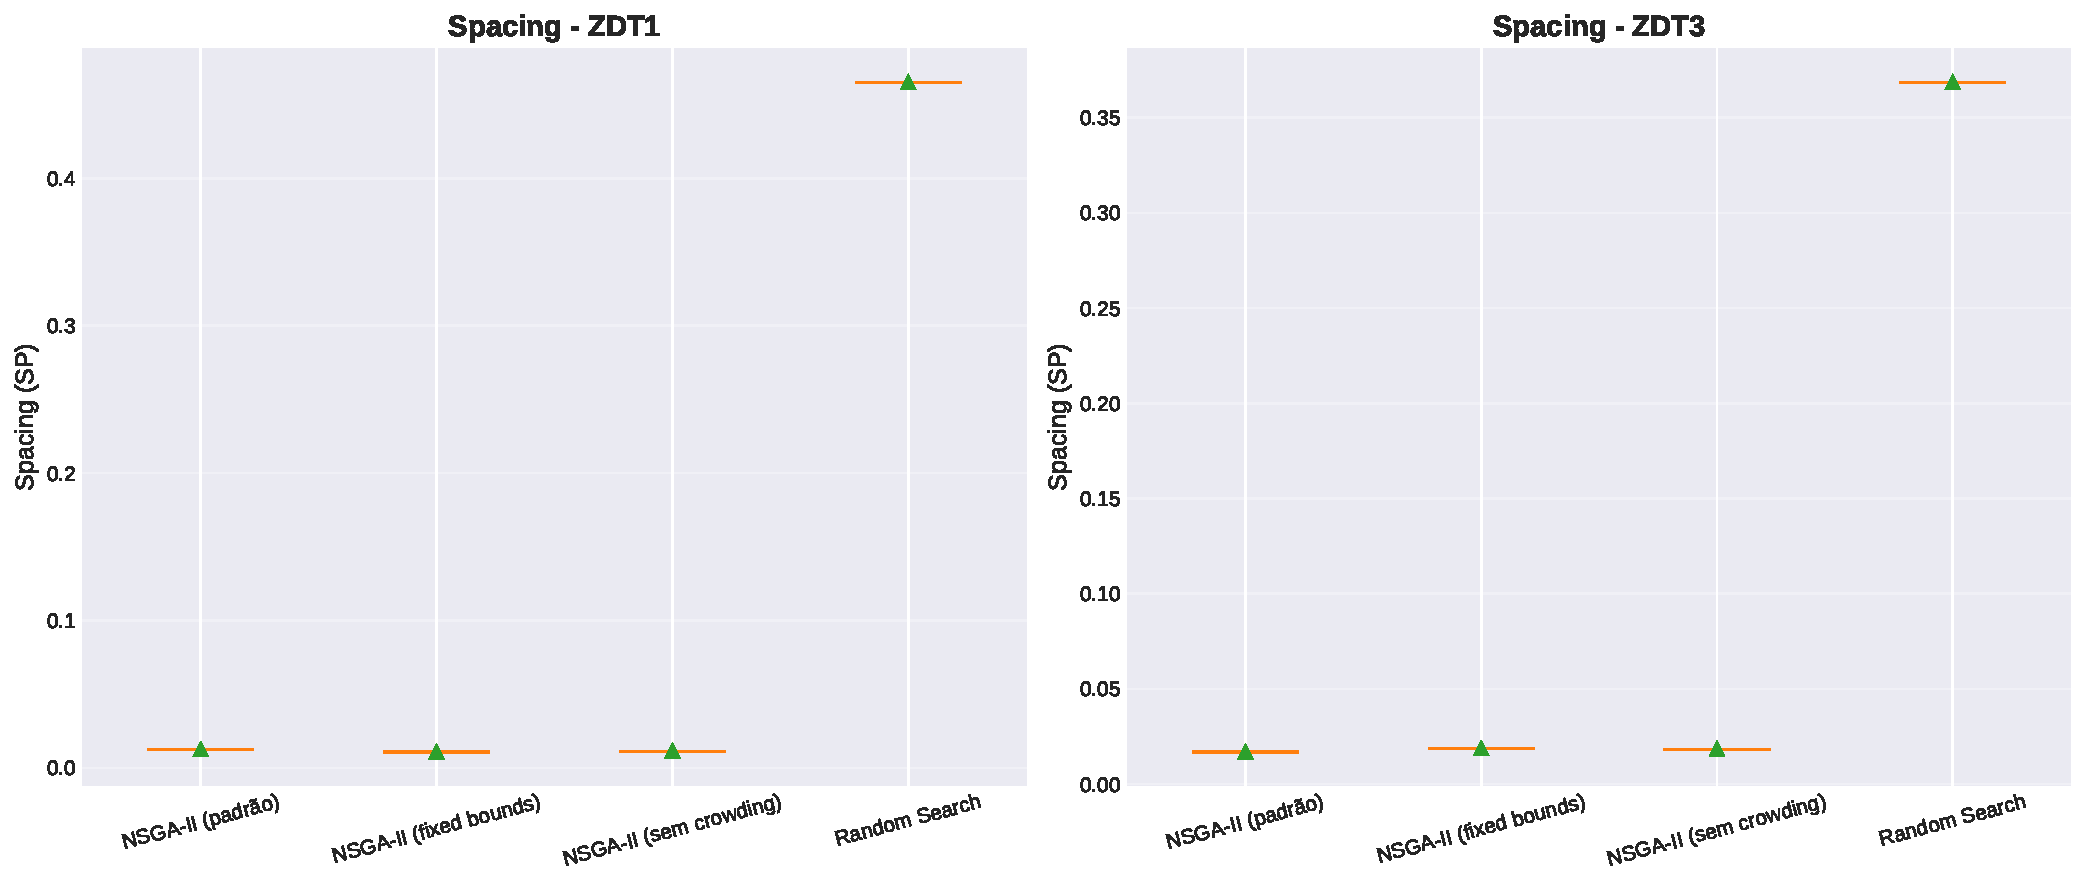
\includegraphics[width=\textwidth]{../plots/D_spacing_boxplots.pdf}
    \caption{Boxplots de Spacing em 10 execuções. NSGA-II com \textit{fixed bounds} apresenta melhor (menor) spacing em ZDT1, enquanto NSGA-II padrão domina em ZDT3. Random Search tem spacing 40× pior, indicando distribuição extremamente irregular.}
    \label{fig:spacing_boxplots}
\end{figure}

\textbf{Observações}:
\begin{itemize}
    \item \textbf{Superioridade NSGA-II}: Spacing 40× melhor que Random Search
    \item \textbf{Fixed bounds em ZDT1}: Ligeira vantagem (13\% melhor) possivelmente devido a normalização mais adequada
    \item \textbf{ZDT3 mais desafiador}: Spacing absoluto ~35\% maior refletindo dificuldade de distribuição em regiões descontínuas
    \item \textbf{Consistência}: Baixa variabilidade intra-algoritmo (CV < 7\%)
\end{itemize}

\subsection{Comparação entre Problemas}

A Figura~\ref{fig:zdt_comparison} facilita comparação direta da performance relativa entre ZDT1 e ZDT3.

\begin{figure}[H]
    \centering
    \includegraphics[width=\textwidth]{../plots/E_zdt1_vs_zdt3.pdf}
    \caption{Comparação de performance entre ZDT1 e ZDT3. \textbf{Superior esquerdo}: Hypervolume. \textbf{Superior direito}: Spacing. \textbf{Inferior}: Comparação de fronteiras de Pareto normalizadas. NSGA-II mantém superioridade consistente em ambos os problemas.}
    \label{fig:zdt_comparison}
\end{figure}

\textbf{Insights principais}:
\begin{itemize}
    \item \textbf{Robustez do NSGA-II}: Performance consistentemente superior independente da topologia
    \item \textbf{Scaling de métricas}: HV absoluto maior em ZDT3 devido a valores negativos de $f_2$
    \item \textbf{Desafio relativo}: Spacing pior em ZDT3 confirma dificuldade adicional de descontinuidade
    \item \textbf{Ineficácia do Random}: Falha categórica em ambos os problemas
\end{itemize}

